\documentclass{article}
\usepackage[utf8]{inputenc}
\usepackage[document]{ragged2e}
\usepackage{algpseudocode}
\usepackage[]{algorithmicx}
\usepackage{amsmath}
\usepackage{amsthm}
\usepackage{amssymb}
\usepackage[]{listings}
\usepackage{graphicx}
\usepackage{hyperref}
\usepackage{flafter}
\usepackage{subfig}
\usepackage{dsfont}
\graphicspath{ {images/} }

\begin{document}

\begin{titlepage}
	\centering
	
\includegraphics[width=0.15\textwidth]{IIIT-B_logo.jpg}\par\vspace{1cm}
	{\scshape\LARGE International Institute of Information Technology, Bangalore \par}
	\vspace{1cm}
	{\scshape\Large Project Strategy Document\par}
	{\Large  DS 707 Data Analytics\par}
	\vspace{1.5cm}
	{\huge\bfseries Blockchain Understanding and Cryptocurrency Analysis \par}
	\vspace{2cm}
	{\Large\itshape Akanksha Dwivedi - MT2016006\par}
	{\Large\itshape Hitesha Mukherjee - MS2016007\par}
	{\Large\itshape Nayna Jain - MS2017003\par}
	{\Large\itshape Tarini Chandrashekhar - MT2016144\par}
	\vfill
	Instructors : \par
	Prof. Ramanathan Chandrashekhar
	\par
	Prof. Uttam Kumar

	\vfill
% Bottom of the page
	{\large \today\par}
\end{titlepage}

\newpage

\tableofcontents

\newpage
\justify

\

\section{Data Understanding}

\subsection{Initial Data Collection }

The source of the data is \textbf{Kaggle}; a featured dataset called Cryptocurrency Historical Prices. It consists of .CSV files of the prices of top cryptocurrencies including Bitcoin, Ethereum, Ripple and Bitcoin cash. For the purposes of exploration, we have initially considered the data on Bitcoin and Ethereum. 
\subsection{Description of data}
The files are basically of two types. One, which contains the seven attributes, captured from \url{coinmarketcap.com}, namely - Date, Open, Close, High, Low, Volume, Market Cap. They describe respectively date, the opening price of the currency, the closing price of the currency, the lowest and highest prices recorded in a day, the total amount of cryptocurrencies swapped in the period of 24 hours, and total evaluation of the currency on a given day. The attributes capture DateTime and numeric data. This file is the same for both Bitcoin and Ethereum dataset.
\begin{equation}
    Market Cap = Price X Circulating Supply
\end{equation}
where Circulating Supply is the best approximation of the number of coins that are circulating in the market and in the general public's hands.
\newline
The second bitcoin file consists of the following 24 handcrafted features, which are :
\begin{itemize}
 
\item Date : Date of observation
\item btc\_market\_price : Average USD market price across major bitcoin exchanges.
\item btc\_total\_bitcoins : The total number of bitcoins that have already been mined.
\item btc\_market\_cap : The total USD value of bitcoin supply in circulation.
\item btc\_trade\_volume : The total USD value of trading volume on major bitcoin exchanges.
\item btc\_blocks\_size : The total size of all block headers and transactions.
\item btc\_avg\_block\_size : The average block size in MB.
\item btc\_n\_orphaned\_blocks : The total number of blocks mined but ultimately not attached to the main Bitcoin blockchain.
\item btc\_n\_transactions\_per\_block : The average number of transactions per block.
\item btc\_median\_confirmation\_time : The median time for a transaction to be accepted into a mined block.
\item btc\_hash\_rate : The estimated number of tera hashes per second the Bitcoin network is performing.
\item btc\_difficulty : A relative measure of how difficult it is to find a new block.
\item btc\_miners\_revenue : Total value of coinbase block rewards and transaction fees paid to miners.
\item btc\_transaction\_fees : The total value of all transaction fees paid to miners.
\item btc\_cost\_per\_transaction\_percent : miners revenue as percentage of the transaction volume.
\item btc\_cost\_per\_transaction : miners revenue divided by the number of transactions.
\item btc\_n\_unique\_addresses : The total number of unique addresses used on the Bitcoin blockchain.
\item btc\_n\_transactions : The number of daily confirmed Bitcoin transactions.
\item btc\_n\_transactions\_total : Total number of transactions.
\item btc\_n\_transactions\_excluding\_popular : The total number of Bitcoin transactions, excluding the 100 most popular addresses.
\item btc\_n\_transactions\_excluding\_chains\_longer\_than\_100 : The total number of Bitcoin transactions per day excluding long transaction chains.
\item btc\_output\_volume : The total value of all transaction outputs per day.
\item btc\_estimated\_transaction\_volume : The total estimated value of transactions on the Bitcoin blockchain.
\item btc\_estimated\_transaction\_volume\_usd : The estimated transaction value in USD value.
\end{itemize}

The dataset file describing Ethereum consists of the following 19 handcrafted features:
\begin{itemize}
    \item Date(UTC) : Date of transaction
    \item UnixTimeStamp : unix timestamp
    \item eth\_etherprice : price of ethereum
    \item eth\_tx : number of transactions per day
    \item eth\_address : Cumulative address growth
    \item eth\_supply : Number of ethers in supply
    \item eth\_marketcap : Market cap in USD
    \item eth\_hashrate : hash rate in GH/s
    \item eth\_difficulty : Difficulty level in TH
    \item eth\_blocks : number of blocks per day
    \item eth\_uncles : number of uncles per day
    \item eth\_blocksize : average block size in bytes
    \item eth\_blocktime : average block time in seconds
    \item eth\_gasprice : Average gas price in Wei
    \item eth\_gaslimit : Gas limit per day
    \item eth\_gasused : total gas used per day
    \item eth\_ethersupply : new ether supply per day
    \item eth\_chaindatasize : chain data size in bytes
    \item eth\_ens\_register : Ethereal Name Service (ENS) registrations per day
\end{itemize}



\subsection{Data Exploration}
Data Exploration involves getting insights from the data using charts and visualizations. As explained in the previous section, there are two types of
datasets i.e. one related to daily trading prices and other giving details on the blockchain characteristics. According to the summary statistics below, the lowest open price has been 68.5 whereas the highest is 4901. which implies that currency has surged very rapidly. From exploratory analytics done, we can see that there hasn’t been much activity in the years 2013 and 2015 while activity has grown in 2014 and it picked lot of action from traders in the years 2016 and 2017.
\begin{figure}

    \centering
    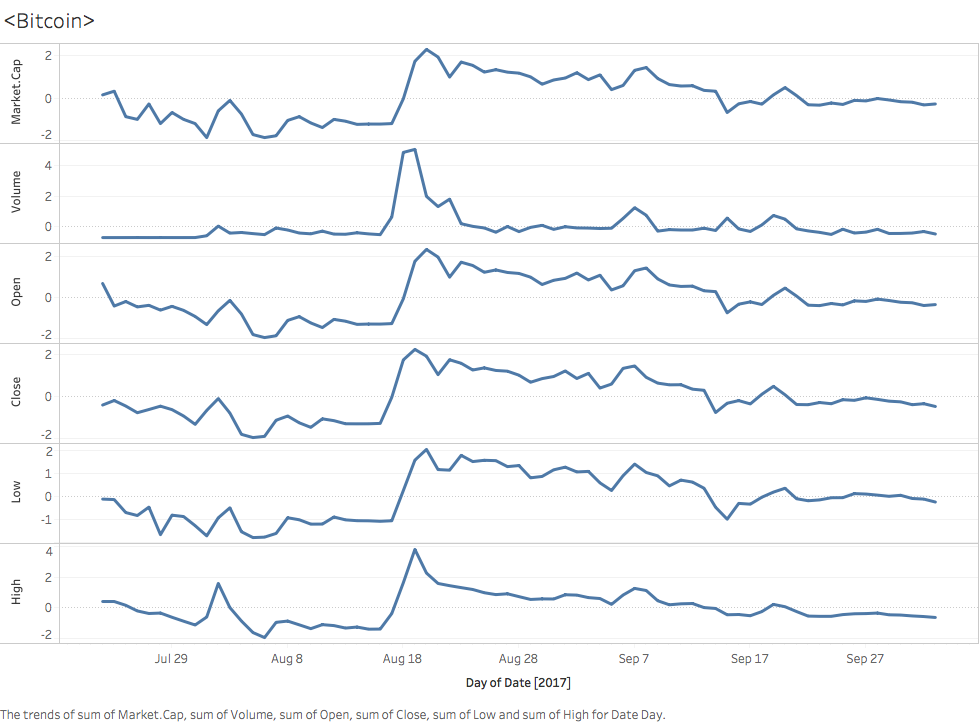
\includegraphics[width = 7cm,height=7cm]{Sheet1.png}
    \caption{Variation of Bitcoin attributes on a daily basis}
    \label{fig:my_label}
    
\end{figure}

\begin{figure}

    \centering
    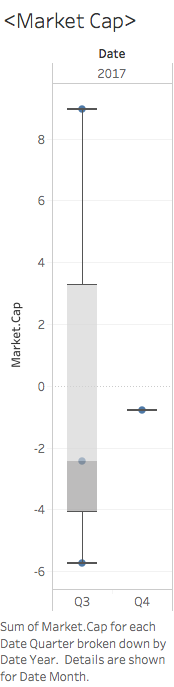
\includegraphics[width = 5cm,height=10cm]{Sheet2.png}
    \caption{Box plot showing Market cap of Bitcoin }
    \label{fig:my_label}
    
\end{figure}


\vfill
\begin{figure}

    \centering
    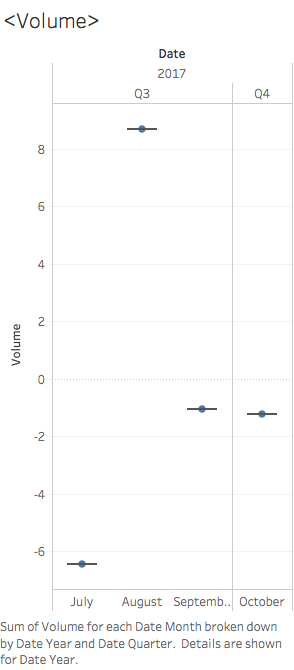
\includegraphics[width = 7cm,height=7cm]{Sheet3.png}
    \caption{Box plot showing Volume trends of Bitcoin}
    \label{fig:my_label}
    
\end{figure}

\vfill
\begin{figure}

    \centering
    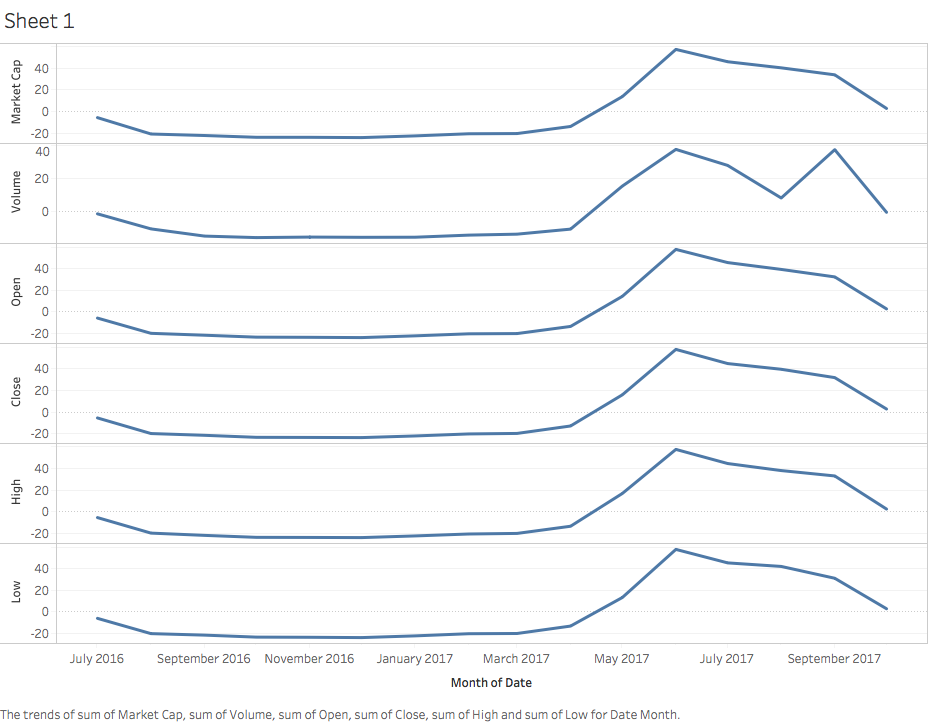
\includegraphics[width = 7cm,height=7cm]{Sheet21.png}
    \caption{Variation of Ethereum attributes on a monthly basis }
    \label{fig:my_label}
    
\end{figure}

\vfill
\begin{figure}

    \centering
    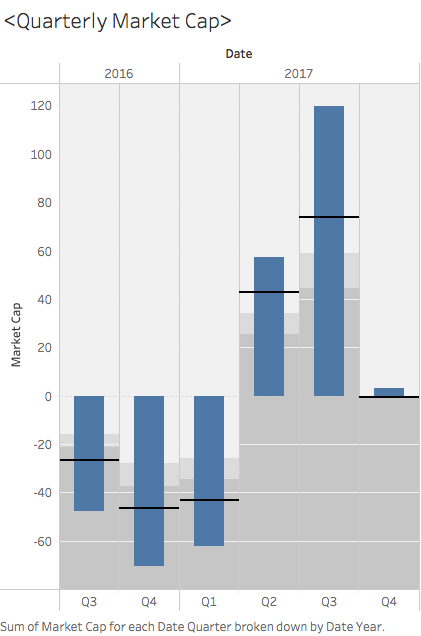
\includegraphics[width = 7cm,height=7cm]{Sheet22.png}
    \caption{Box plot showing quarterly market cap on Ethereum}
    \label{fig:my_label}
    
\end{figure}

\vfill
\begin{figure}

    \centering
    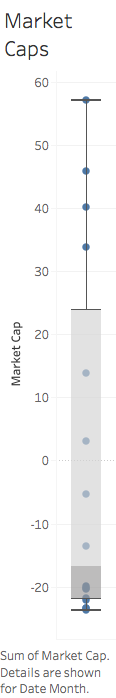
\includegraphics[width = 5cm,height=10cm]{Sheet23.png}
    \caption{Box plot showing Volume trends of Ethereum}
    \label{fig:my_label}
    
\end{figure}
\newpage
Figure 1 - shows that all the 6 attributes vary almost similarly with time in case of bitcoin.\newline
Figure 2 - This box plot shows the variation of market cap values, while there lie 2 outliers for the first quartile, and there isn't enough data to derive a range for the second quartile. \newline
Figure 3 - This box plot shows that that volume values don't exist as a range for Bitcoin, but exist as almost absolute values for the months of the year.\newline
Figure 4 - Much like in case of Bitcoin, the above graph confirms that Ethereum attributes vary almost similarly with each month.\newline
Figure 5 - This box plot shows the variation in the market cap of each quarter of Ethereum and there seem to be no outliers.\newline
Figure 6 - This box plot shows that that volume values don't exist as a range for Ethereum, but exist as almost absolute values for the quarters.\newline

The box plots on volume and market cap for both Bitcoin and Ethereum give us a valuable insight. The Market Cap value exists as a range for different months of the year, whereas Volume values are absolutes. This shows that while Market cap differs and is volatile because of the volatility in the pricing of the cryptocurrencies, the Volume remains constant for a given time frame, because it is the average amount of crytocurrency swapped in a day. This value doesn't differ rapidly for a given time frame.


This data can be used to:
\begin{itemize}
\item Predict cryptocurrency price in the future.

\item This also helps to analyse the surge in the market.

\item The comparision of this chart between different cryptocurrencies will help us to compare them and find the popular cryptocurrency and the one which has got the highest price.

We have also plotted the box plot and see there are lot of outliers, that is because there has been surge recently in crypto currency especially bitcoin trading activities.These outliers also help to analyse any anamolies. 

For a given continuous variable, outliers are those observations that lie outside 1.5 * IQR, where IQR, the ‘Inter Quartile Range’ is the difference between 75th and 25th quartiles. Look at the points outside the whiskers in below box plot.
\end{itemize}


\begin{figure}
    \centering
    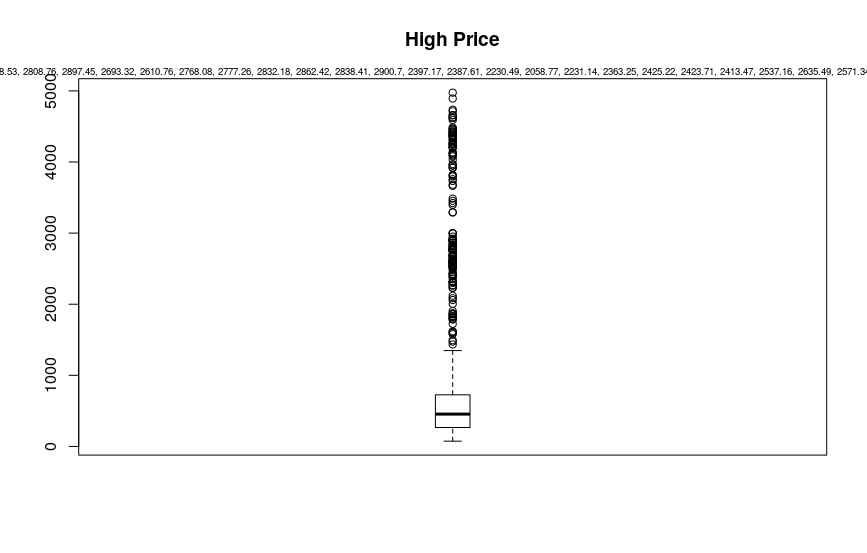
\includegraphics[width=\linewidth]{bitcoin_price_highprice_boxplot}
    \caption{Univariate Approach : High \textunderscore Price}
    \label{fig:my_label}
\end{figure}




\begin{figure}
    \centering
    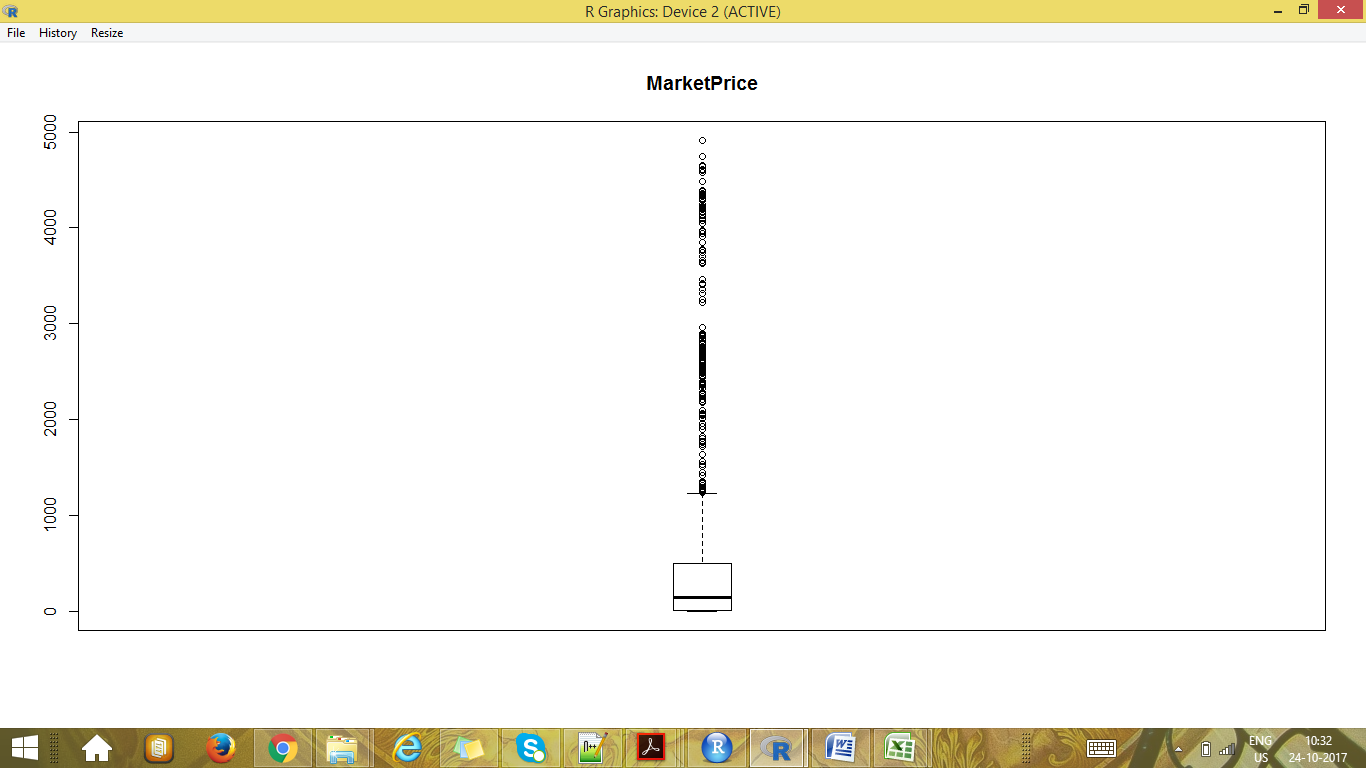
\includegraphics[width=\linewidth]{bitcoin_price_marketprice_boxplot}
    \caption{Bitcoin\textunderscore Market\textunderscore Price\textunderscore Outliers}
    \label{fig:my_label}
\end{figure}



\begin{figure}
    \centering
    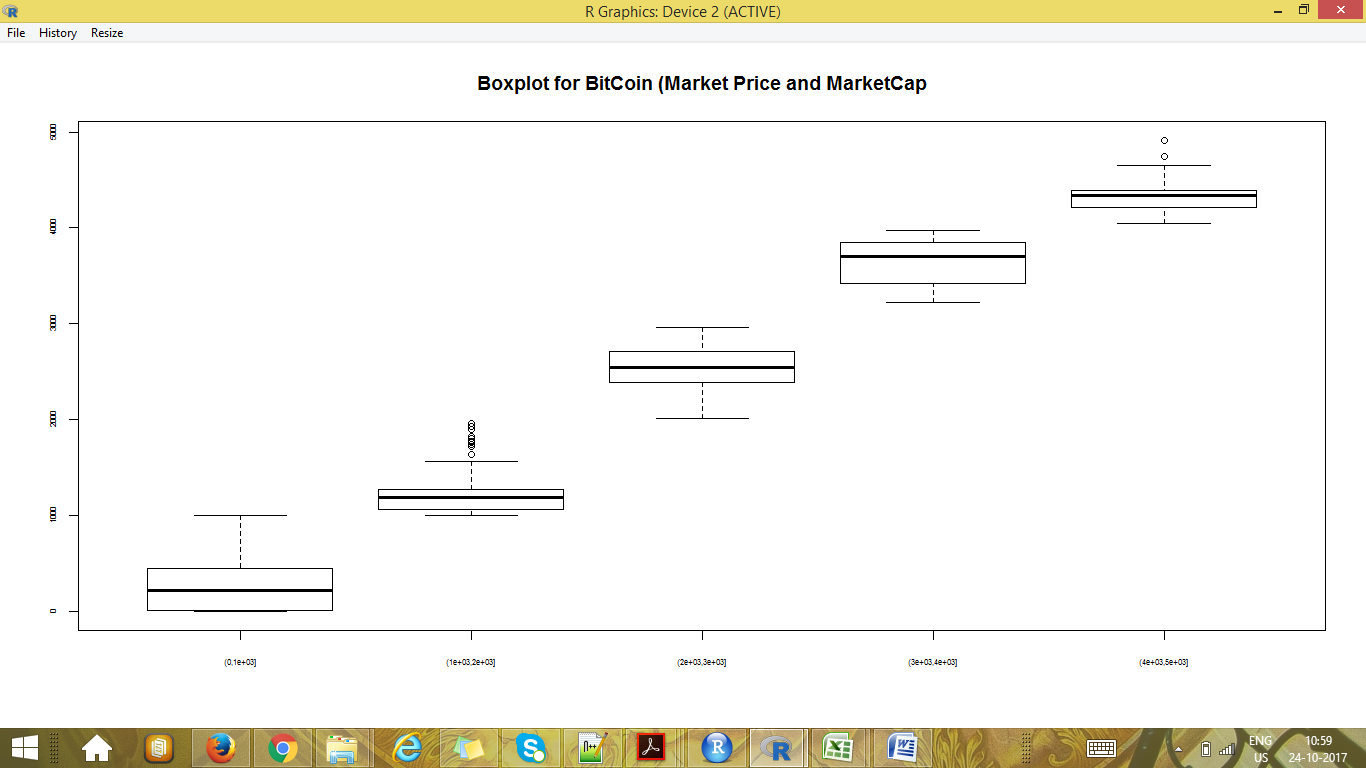
\includegraphics[width=\linewidth]{bitcoin_dataset_marketprice_cap_boxplot}
    \caption{Bivariate Approach : Bitcoin Market Price and Market Cap Outlier}
    \label{fig:my_label}
\end{figure}


\begin{figure}
    \centering
    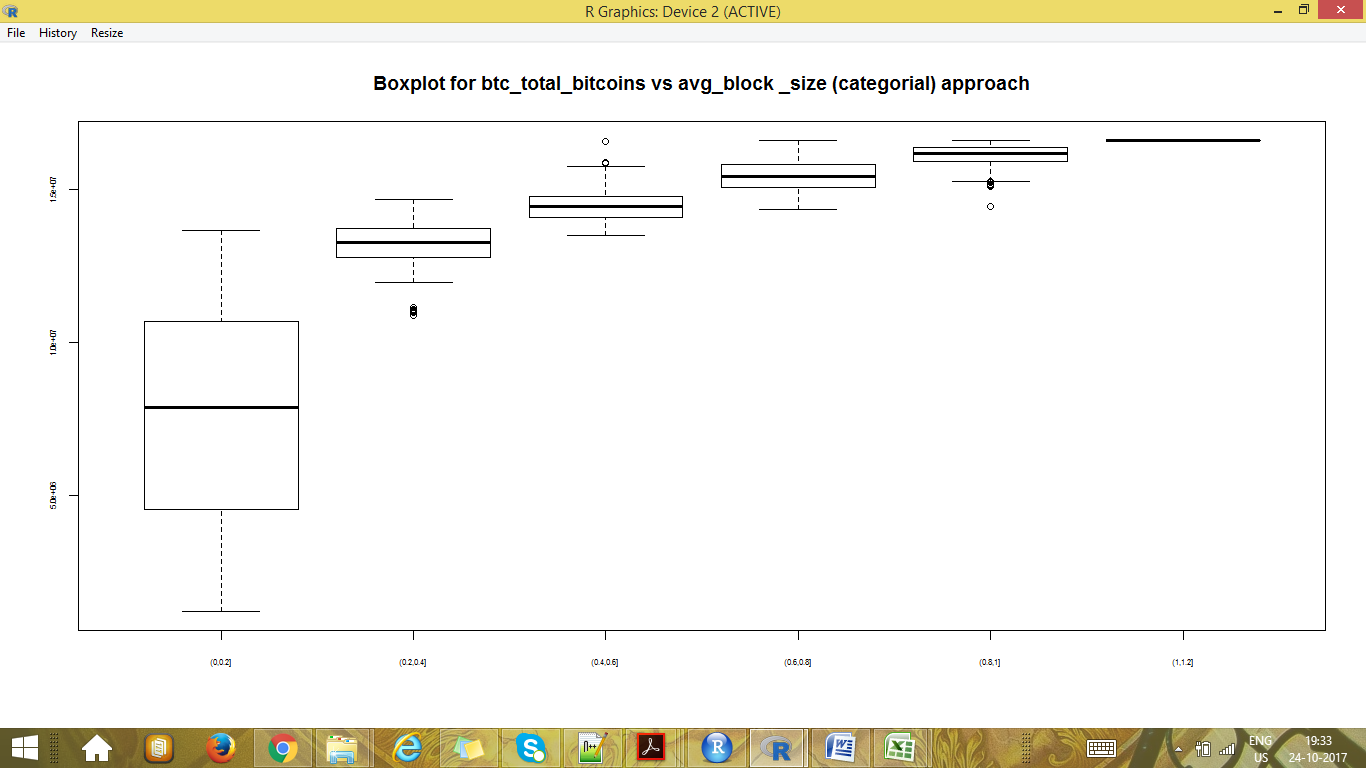
\includegraphics[width=\linewidth]{bitcoin_dataset_btc_total_bitcoins_avg_block_size_boxplot}
    \caption{Bivariate approach : Boxplot for Total Bitcoins and AvgBlockSize}
    \label{fig:my_label}
\end{figure}
\newpage
Figure 7 - The figure captures outliers on High Price for BitcoinPrice.csv. We are plotting only one column or attribute “High” present in the BitcoinPrice.csv.
\newline Figure 8 - The figure captures outliers on Market price for BitcoinDataset.csv. We are plotting only one column or attribute “MarketPrice” present in the BitcoinDataset.csv
\newline Figure 9 - This figure captures outliers on Market Price and Market Cap for bitcoin datset.csv. We observe outliers which show up as dots.
\newline Figure 10 - This figure captures outliers on Total Bitcoins and Average block size for bitcoin datset.csv. We observe outliers which show up as dots.BoxPlot for btc\textunderscore total\textunderscore bitcoins versus avg \textunderscore block\textunderscore size for bitcoin dataset.csv. We observe there are two outliers which show up as dots outside the whiskers of box plot.

\subsection{Data Quality Verification}

Data has been verified to identify:
\begin{itemize}
\item  Missing data: We identified that bitcoin price dataset has missing values for Volume for 7 months of Year 2013. It amounts to around 15\% of the data. We also found that bitcoin dataset contains around 27 missing values, which was only around 0.92\% of the total dataset.

\item Data Errors: The dataset does not have any numeric errors. Further, there is no text or factor data, so there are no typographical errors.

\item Measurement Errors: There is single source of data and is based on single measurement scheme, thereby no measurement errors recorded.

\item Coding inconsistencies: Since the data is from single source, there are no coding inconsistencies. Further, we have single format of files i.e. csv, all following the similar delimiter scheme.

\item Bad Metadata: Metadata is from standard terminology, hence no bad metadata issues.
    
\end{itemize}
We observed that the Price data is fit to see the volatility trend of crypto currency. Volume and Market capitalization data will help in creating models for
predicting future prices. Since the data in different attributes are of different units, it needs normalization. The data is clean and consistent, however one of the attributes in every file has missing values. So, we employed \textbf{mice} package to predict the missing values. We did not encounter any data errors, spelling inconsistencies or bad metadata in the the dataset.

\begin{figure}
\centering
\begin{minipage}{.5\textwidth}
  \centering
  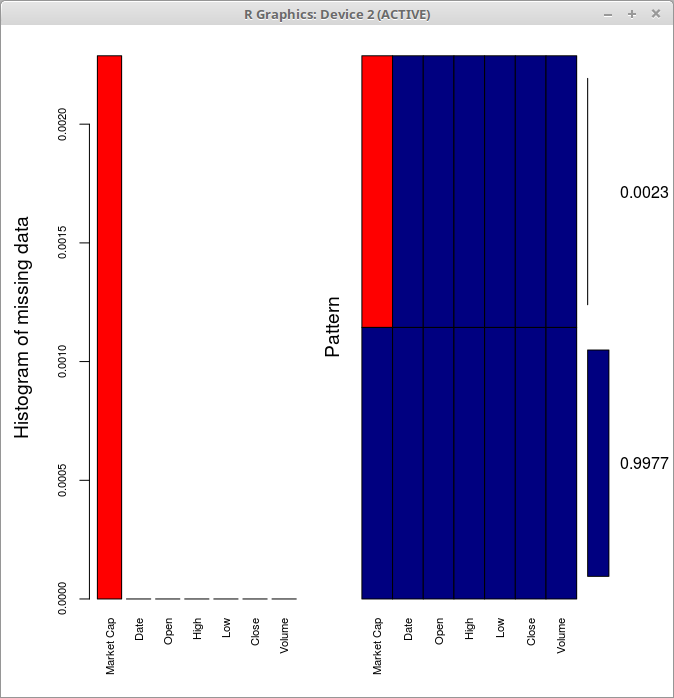
\includegraphics[width=.8\linewidth]{ethereum_classic_price_missing}
  \captionof{figure}{Percentage of missing values in Ethereum Classic Price Dataset}
  \label{fig:test1}
\end{minipage}%
\begin{minipage}{.5\textwidth}
  \centering
  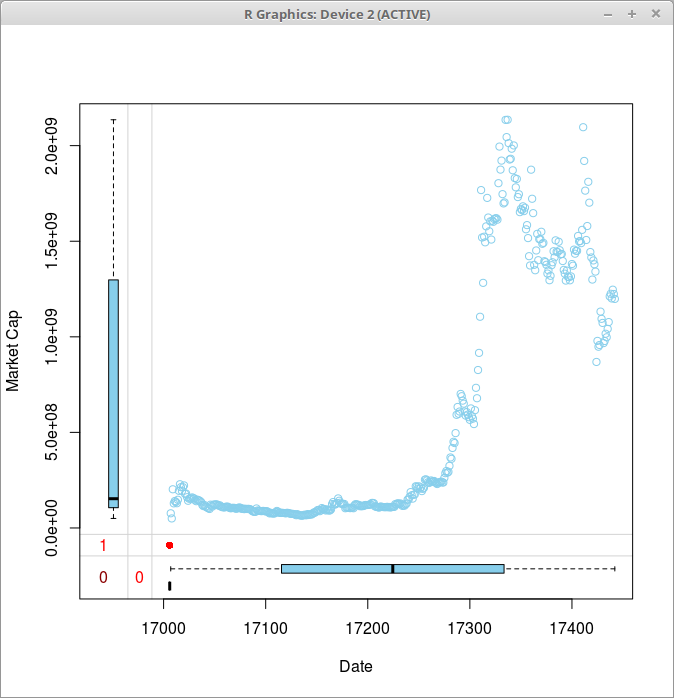
\includegraphics[width=.8\linewidth]{eth_classic_price_missing}
  \captionof{figure}{Box plot of missing attribute with Date column}
  \label{fig:test2}
\end{minipage}
\end{figure}

\begin{figure}
\centering
\begin{minipage}{.5\textwidth}
  \centering
  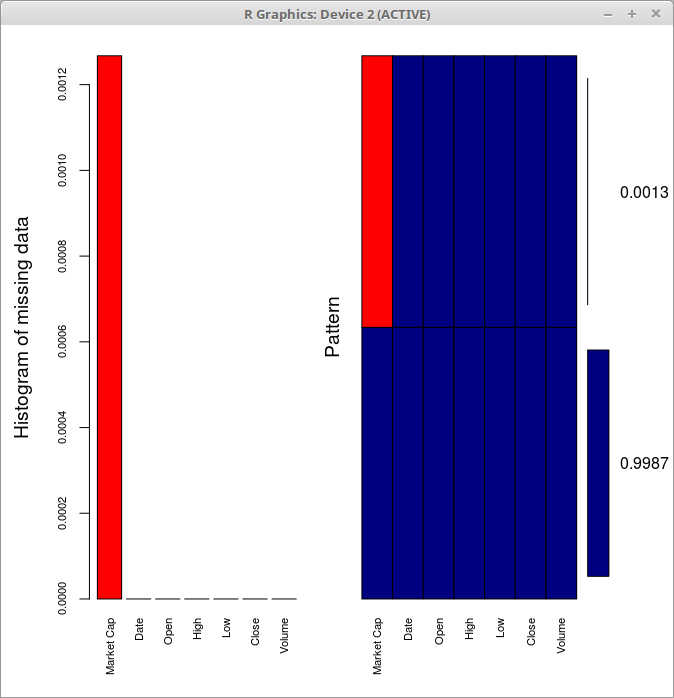
\includegraphics[width=.8\linewidth]{eth_price_missing}
  \captionof{figure}{Percentage of missing values in Ethereum Price Dataset}
  \label{fig:test1}
\end{minipage}%
\begin{minipage}{.5\textwidth}
  \centering
  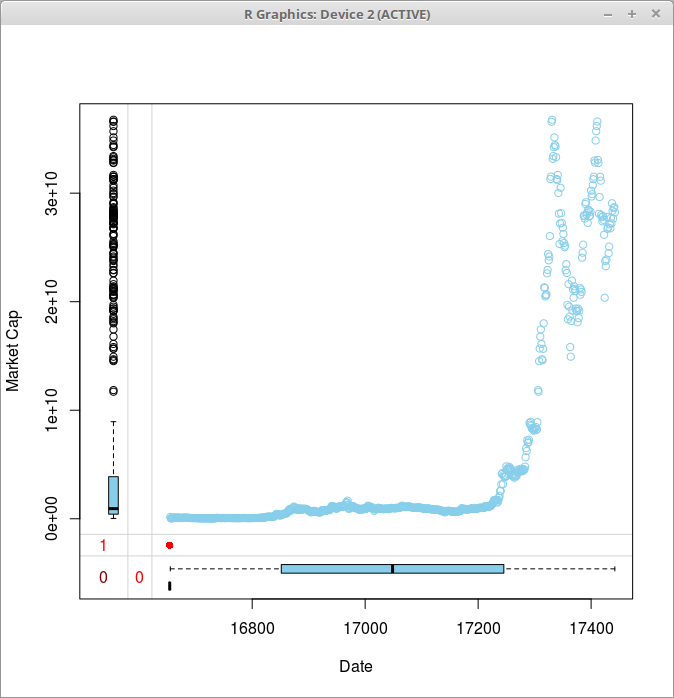
\includegraphics[width=.8\linewidth]{eth_price_missing_box_plot}
  \captionof{figure}{Box plot of missing attribute with Date column}
  \label{fig:test2}
\end{minipage}
\end{figure}

\begin{figure}
\centering
\begin{minipage}{.5\textwidth}
  \centering
  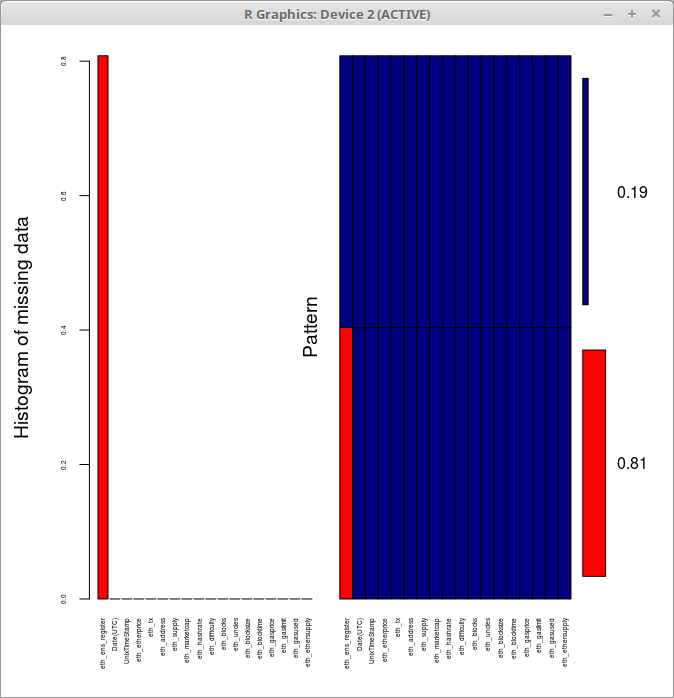
\includegraphics[width=.8\linewidth]{eth_dataset_missing}
  \captionof{figure}{Percentage of missing values in Ethereum Dataset}
  \label{fig:test1}
\end{minipage}%
\begin{minipage}{.5\textwidth}
  \centering
  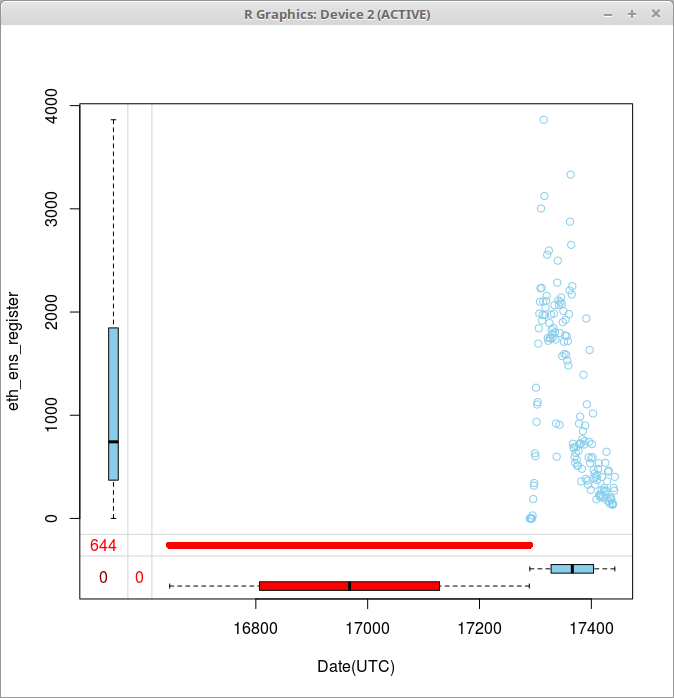
\includegraphics[width=.8\linewidth]{eth_dataset_missing_box_plot}
  \captionof{figure}{Box plot of missing attribute with Date column}
  \label{fig:test2}
\end{minipage}
\end{figure}

\begin{figure}
\centering
\begin{minipage}{.5\textwidth}
  \centering
  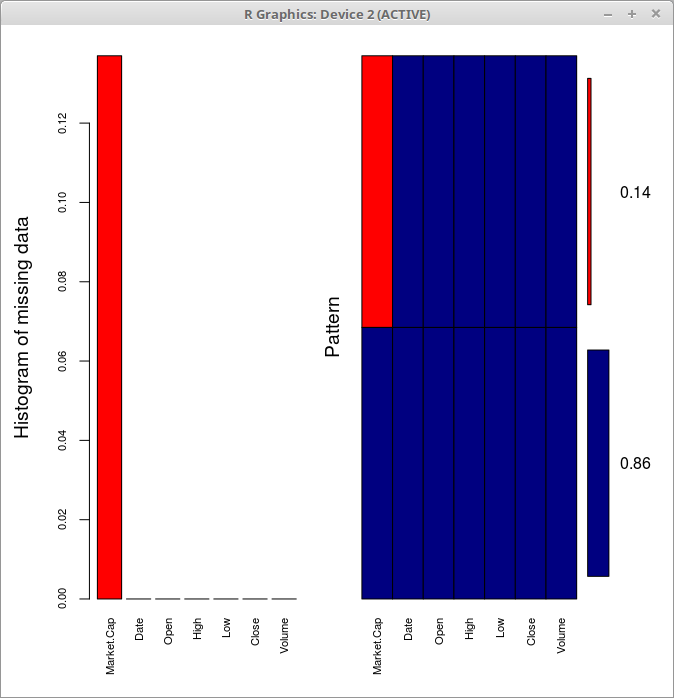
\includegraphics[width=.8\linewidth]{btc_cash_price_missing}
  \captionof{figure}{Percentage of missing values in Bitcoin Cash Price Dataset}
  \label{fig:test1}
\end{minipage}%
\begin{minipage}{.5\textwidth}
  \centering
  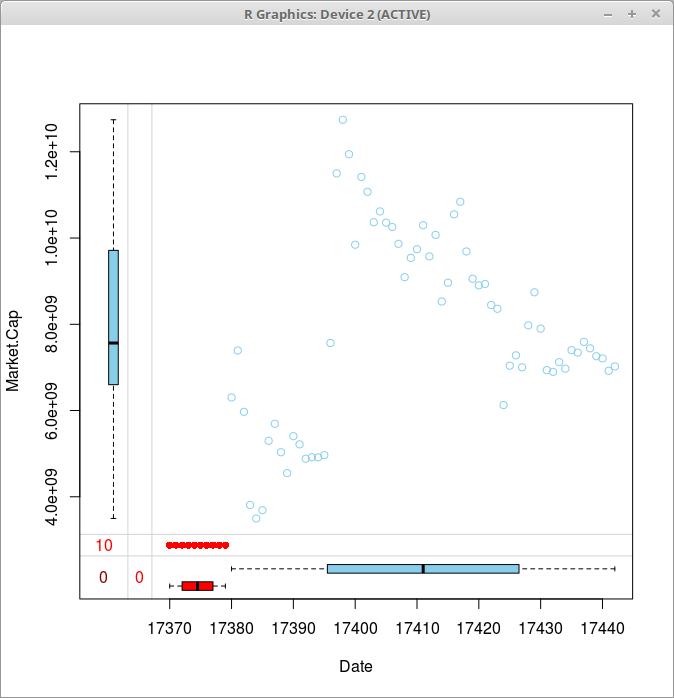
\includegraphics[width=.8\linewidth]{btc_cash_price_missing_box_plot}
  \captionof{figure}{Box plot of missing attribute with Date column}
  \label{fig:test2}
\end{minipage}
\end{figure}

\begin{figure}
\centering
\begin{minipage}{.5\textwidth}
  \centering
  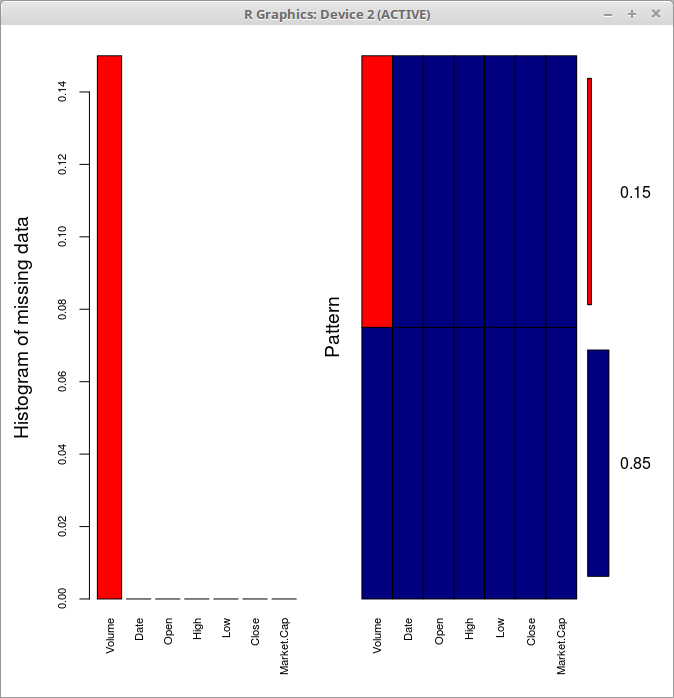
\includegraphics[width=.8\linewidth]{btc_price_missing}
  \captionof{figure}{Percentage of missing values Bitcoin Price Dataset}
  \label{fig:test1}
\end{minipage}%
\begin{minipage}{.5\textwidth}
  \centering
  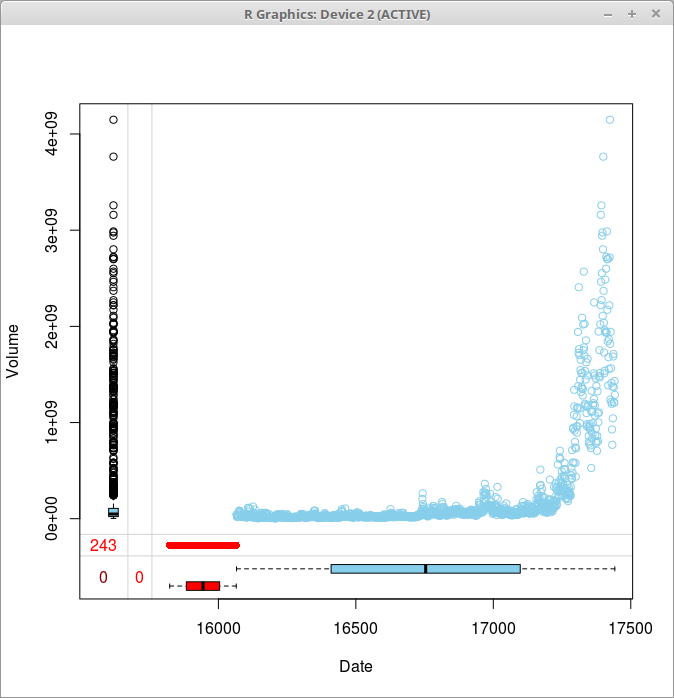
\includegraphics[width=.8\linewidth]{btc_price_missing_box_plot}
  \captionof{figure}{Box plot of missing attribute with Date column}
  \label{fig:test2}
\end{minipage}
\end{figure}

\begin{figure}
\centering
\begin{minipage}{.5\textwidth}
  \centering
  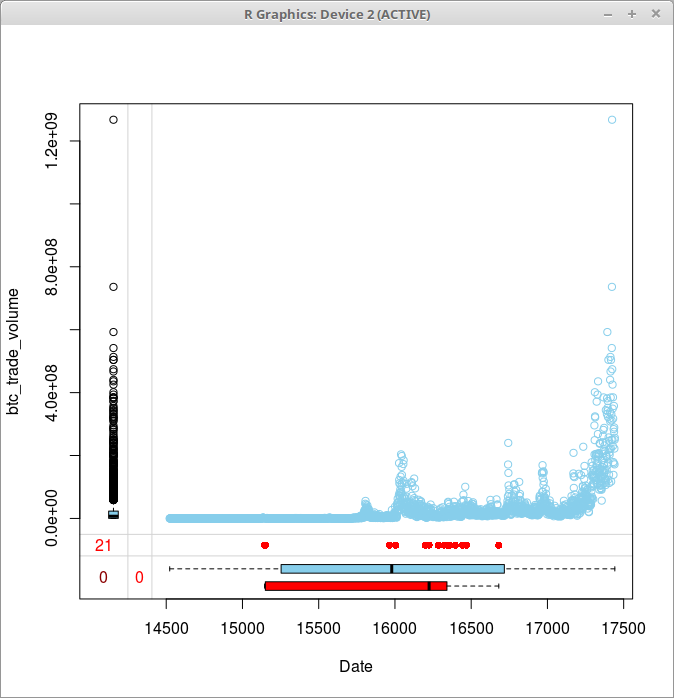
\includegraphics[width=.8\linewidth]{btc_dataset_missing}
  \captionof{figure}{Percentage of missing values in Bitcoin Dataset}
  \label{fig:test1}
\end{minipage}%
\begin{minipage}{.5\textwidth}
  \centering
  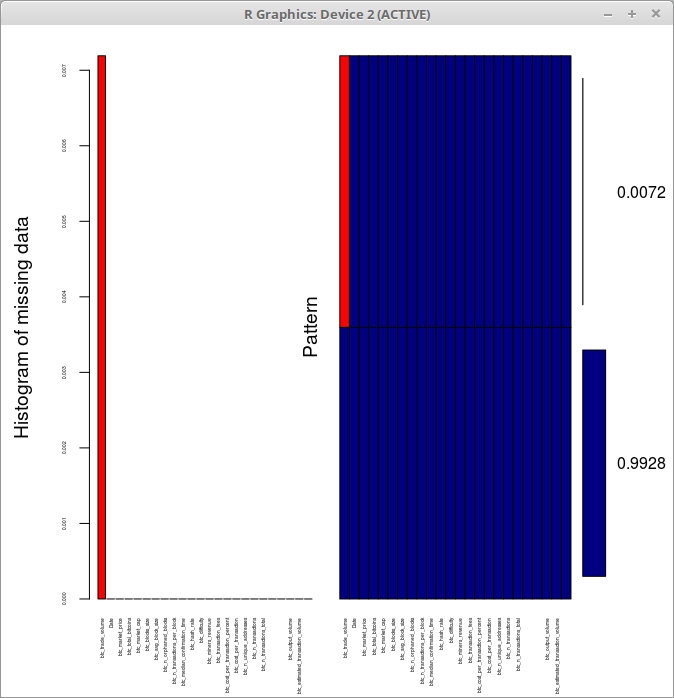
\includegraphics[width=.8\linewidth]{btc_dataset_missing_box_plot}
  \captionof{figure}{Box plot of missing attribute with Date column}
  \label{fig:test2}
\end{minipage}
\end{figure}

\newpage
Figure 11-24 describes the overall percentage of missing values for all the six datasets used for this exploration endeavour. The Histogram shows the different attributes contributing in the missing values. The box plot takes two attributes in account with their corelation with each other, one of which has been fixed as Date feature. The other attribute is chosen, contributing most to the missing values. As the two box plots (red and blue in color) are not similar in size with each other, thereby suggesting that the NA values in the dataset are not missed at random.


\begin{figure}
    \centering
    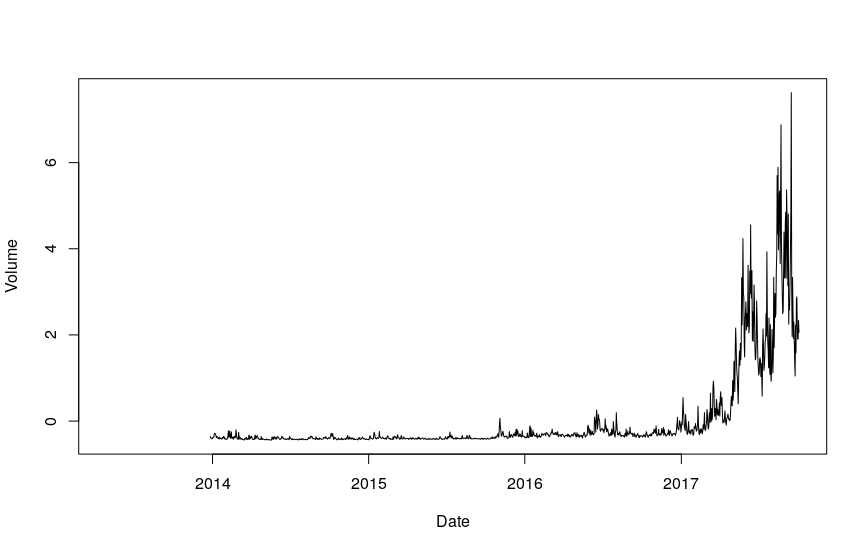
\includegraphics[width=\linewidth]{bitcoin_price_with_missing_values}
    \caption{Bitcoin Volume Against Date}
    \label{fig:my_label}
\end{figure}



\begin{figure}
    \centering
    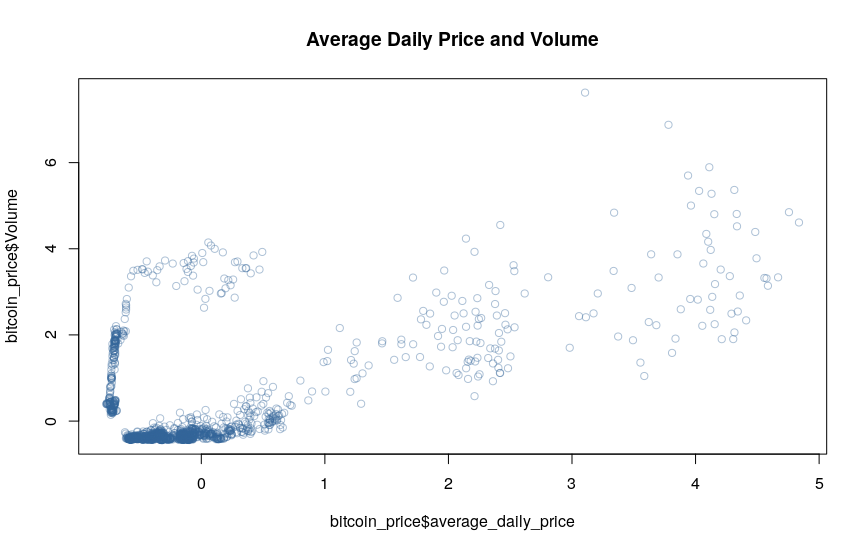
\includegraphics[width=\linewidth]{AverageDailyPrice_Volume_AfterFillingMissing.png}
    \caption{Using Linear Regression}
    \label{fig:my_label}
\end{figure}

\newline
 

\begin{figure}
    \centering
    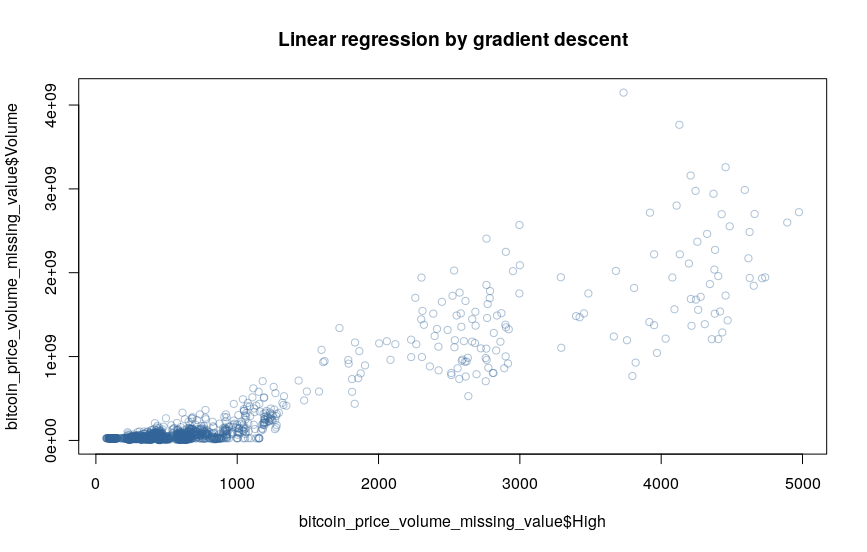
\includegraphics[width=\linewidth]{Volume_After_Filling_Missing_Value.png}
    \caption{Using Nearest Neighbour Mean}
    \label{fig:my_label}
\end{figure}



\begin{figure}
    \centering
    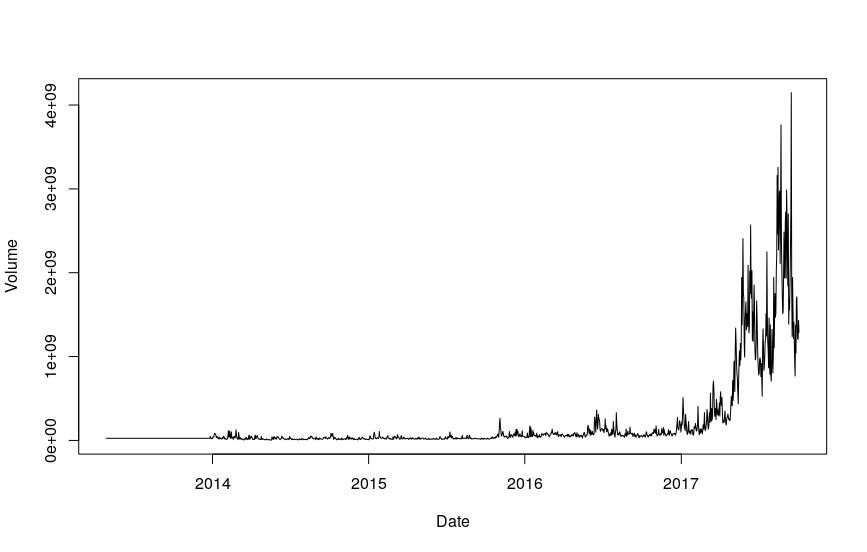
\includegraphics[width=\linewidth]{MissingValue_Against_Date.png}
    \caption{Missing Values Against Date after Filling}
    \label{fig:my_label}
\end{figure}

\newpage
The above figure shows that missing values are in trend after filling.
\newline Figure 25 -  This figure shows that volume has been consistent across the whole year of 2014 with slight peaks. We have used two ways to identify the missing values. After that we plotted again to verify our prediction.
\newline Figure 26 - From our domain information, we consider that volume of the price might get impacted based on its average daily price.We calculate the average daily price by taking average of daily High and Low. 
\newline Figure 27 - It can be seen that the trend in volume of trading has been consistent across year 2014. So, we applied the method where we can take the mean of similar class and use that mean value to try and fill the missing values. Thus, we calculate the mean for Dec 2013 to Dec 2014 and then use that mean to fill the missing value in Excel.
\newline Figure 28 - This shows the chart after filled missing values using this method. If we compare above figures, we can see that in this particular case, simple regression mechanism didn't predict the values so correctly, but using the mean from nearest neighbour was more consistent. Hence, we used hybrid regression and decision trees mechanism to predict the missing values, excluding the Date column.

\newpage
\section{Data Preparation}

\subsection{Selection of Data}
There are two types of missing data:
\begin{itemize}
    
\item MCAR: Missing Completely At Random. This is the desirable scenario in case of missing data.
\item MNAR: Missing Not At Random. Missing not at random data is a more serious issue and in this case it might be wise to check the data gathering process further and try to understand why the information is missing. For instance, if most of the people in a survey did not answer a certain question, why did they do that? Was the question unclear?
\end{itemize}
Assuming data is MCAR, too much missing data can be a problem too. Usually a safe maximum threshold is 5\% of the total for large datasets. If missing data for a certain feature is more than 5\% then we probably should leave that feature out. We therefore check for features (columns) and samples (rows) where more than 5\% of the data is missing. Here, the missing value percentage is less than 5\% for all the attributes except one, so we keep them. However, for the attribute eth\_ens\_register approximately 81\% values are missing. So, we ignored this dataset until we gather more measurements.

\subsection{Cleaning \& Formatting of Data}
The cleaning and formatting of data follows a certain order:
\begin{itemize}
    \item We first change the date into proper format, according to the input file. 
    \item We calculate the number of NA(missing) values and get to know their pattern.
    \item Then we employ imputation. Imputation of missing values refers to replacing missing data with substituted values. In R, we use the mice package to do the same. The mice() function takes three parameters - number of imputed datasets (default value is 5), method of imputation, maximum number of iterations, and seeds(for random number generation).
\end{itemize}


\subsection{Construction \& Integration Of Data}
\begin{itemize}
\item The attributes Open, Close, High and Low attributes are inherently useful in price prediction. However, we have derived an attribute from the former called average price, which can be used in the prediction task. Average price suggests investor to decide whether to trade or not, which might impact thevolume. However, if the volatility is very high, it may not give right prediction.
We have calculated average daily price using (Low + High)/2 for bitcoin dataset.
\item We merged the above imputed dataset with the original dataset. 
\item Furthermore, for proper formatting, we add the proper date column and reorder the columns once again.
\item Lastly, we normalised the dataset.
\end{itemize}

\end{document}